\documentclass{article}

\usepackage{xeCJK}

% Formatting
\usepackage{geometry}
\usepackage{titling}
\usepackage{parskip}
\usepackage{float}
\usepackage{tocloft}

% Figures
\usepackage{graphicx}
\usepackage{tikz}
\usepackage{pgfplots}
\usepackage{subcaption}

% Math formulas
\usepackage{amsmath}
\usepackage{esint}

% Hyper refs
\usepackage[hidelinks]{hyperref}

% Bibliography
\usepackage[style=authoryear,backend=bibtex]{biblatex}
\usepackage{filecontents}
% Enlarge the outer brackets of nested formulae.
\delimitershortfall=-1pt

% Bibliography.
\bibstyle{eg-alpha-doi}

% Pseudo code.
\lstdefinestyle{pseudo}{
	mathescape=true,
	extendedchars=true,
	frame=tB,
	breaklines=true,
	tabsize=2,
	numbers=left,
	numberstyle=\tiny,
	basicstyle=\scriptsize,
	keywordstyle=\color{black}\bfseries\em,
	keywords={
		input, output,
		function, datatype,
		return, yield, continue, break
		for, foreach, while,
		do, in, done,
		in, on, from, to,
		if, else,
		begin, end,
		new, delete,
		add, apply,
	},
	numbers=left,
	xleftmargin=.04\textwidth,
}
\newenvironment{keywords}{
	\begin{paragraph}{Keywords}
}{
	\end{paragraph}
}

\title{A Generic Monte-Carlo Framework for Real-time Simulation of Rigid Body Motion Through Force Fields}
\author{Nianyi Wang}
\date{\today}

\addbibresource{references.bib}

\begin{document}

\maketitle

\begin{abstract}[Abstract]
	Lorem ipsum.
\end{abstract}

\begin{keywords}
	physical simulation;
	Monte-Carlo;
	force field;
	rigid body
\end{keywords}

\section{Introduction}

In real-time applications like video games, it is sometimes required to simulate the physical motion of objects moving through physical fields, such as how a light object would float due to the buoyancy force caused by the water body.
With normal methods, it is necessary to make queries to the geometrical shape of the simulated object frequently, usually many times per frame, to ensure the preciseness of the simulation.
However, most common game engines don't provide easy interfaces for geometrical shapes due to the consideration of runtime performance, and it'd be easy to run into performance issues if one were to implement these queries from scratch.

In this article we propose a generic framework to achieve this kind of simulation in a unified way based on the Monte-Carlo method.
It exposes an easy set of interfaces that is left for downstream developers to customize for the desired kind of physical field;
it is also possible to tweak the parameters to balance between simulation quality and performance.

The idea of this article originates from simulating the buoyancy behavior of objects submerged in water, so we will be introducing our method mainly with water simulation as a concrete situation.

\section{Related Works}

Speaking in the field of water simulation, the exisiting methods could be divided into two parties: the Lagrangian method, which models water into individual particles and simulates the physical behavior of each one, and the Eulerian method, which treats the entire water body as a continuous region and represents it as a field \cite{GOU09}.
Most of the researches on these methods focus on simulating either water itself or the two-way coupling between water and submerged objects,
but in this research, we mainly focus on the one-way effect caused on the objects by the field, the Lagrangian method would have little contribution to our goal, so we will scope to only the Eulerian method.

The first simulation algorithm for solid-fluid coupling that is based entirely on Eulerian fluid is \cite{teng2016eulerian}.
This plain algorithm could achieve the goal of recreating the realistic physical behaviors well, but is too slow for real-time applications, as it would take seconds for a single frame to be rendered.

\cite{GER13} and \cite{BAJ20} proposed algorithms for real-time simulation, but both are based on proxy-based approximation of different manners.
\cite{GER13} takes the entire fluid volume as the induced field of a
limited amount of "panels"---essentially generating seeds at certain location that represent the surrounding fluid motion in their adjacent spaces.
It is cheap enough to run at a real-time scale in a 2D game, but sacrifices the accuracy from reducing the freedom of the fluid’s behavior.
\cite{BAJ20} disects the submerged objects into inter-connected virutal containers.
When an object is submerged in water, the algorithm would simulate the gradual change of water floating into the containers, thus creating a sinking effect.
This algorithm is also cheap enough to be run in real-time, but requires all objects that would be submerged to be equipped with manually-configured virtual container setup.

There were two Monte-Carlo fluid simulation algorithm (\cite{sugimoto2024velocity} and \cite{rioux2022monte}) proposed in recent years, but they are all fluid solvers, not capable for handling the physical effect on objects moving through.

\section{Method}

Rigid bodies are treated as point masses in many cases because the precise shapes don't matter, but in our case, they do matter.
Take the following series of illustration as an example:
When a wooden plank falls into water, one side of it first touches the water, and the buoyancy force causes a torque, causing the plank to pitch.
Had the plank taken as a simple point mass, the torque couldn't have been reflected, and also the buoyancy force would have only taken effect after the center of mass of the plank passes the water surface.

\begin{figure}[h]
	\def\ih{1in}
	\centering
	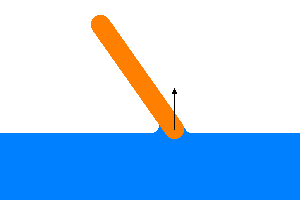
\includegraphics[height=\ih]{../Thesis/figures/stages-of-a-plank-falling-into-water/1.png}
	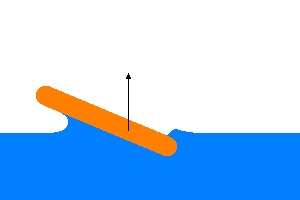
\includegraphics[height=\ih]{../Thesis/figures/stages-of-a-plank-falling-into-water/2.png}
	
\includegraphics[height=\ih]{../Thesis/figures/stages-of-a-plank-falling-into-water/3.png}
	\caption{The stages of a plank falling into water.}
\end{figure}

To ensure that we could get the correct result, we should take the entire volume of the rigid body into consideration.
This sounds computational heavy, but luckily there is the \emph{divergence theorem} to simplify the case:
The integral of the divergence of a vector field ($\mathbf{F}$) over a volume ($V$) is equal to the flux of the field on the boundary of the volume (\ref{formula:divergence-theorem}).

\begin{equation}
	\iiint_{V}(\nabla\cdot\mathbf{F})\mathrm{d}V
	=
	\oiint_{\partial V}\left(\mathbf{F}\cdot\hat{\mathbf{n}}\right)\mathrm{d}\partial V
	.
	\label{formula:divergence-theorem}
\end{equation}

This theorem could leads to several important laws in physics that's related to our topic, such as \emph{Archimedes' principle} in fluid mechanics and \emph{Gauss's law} in electromagnetism.

\section{Applications}

\section{Limitation and Future Work}

Jitter.

GPU acceleration.

\section{Conclusion}

\section*{Acknowledgement}

This is the first time I have ever written a serious academical article.
It is guaranteed that there will be naive mistakes all over the place.
Please excuse me, thou reader.
If thou hast spotted any mistake, please feel free to contact me at \url{wangnianyi2001@outlook.com}.
My apologies in advance!

Thanks to the team of my graduation project, \emph{Nani Core} (\url{https://github.com/nani-core}).
The idea of this article rose when I was making the water system in the project.
They established the possibilty for this article to happen.
Special thanks to 陈恩晖 (Omnisch) and 张嘉玥 (Limko).
They are two really, really reliable co-workers and good friends of mine.
They have given me the greatest mental and physical support on the project, and an unforgetful memory in my graduation year.

% A sample project of the simulation experiment is published at \url{https://github.com/WangNianyi2001/Water-Simulation-2024}.

\printbibliography

\end{document}